\documentclass[10pt, conference, compsocconf]{IEEEtran}

\usepackage{url}
\usepackage{flushend}
\usepackage{mdwlist} % description itemize
\ifCLASSOPTIONcompsoc
% requires cite.sty v4.0 or later (November 2003)
\usepackage[nocompress]{cite}
\else
\usepackage{cite}
\fi
\usepackage{listings}
\usepackage[utf8]{inputenc}
\usepackage{graphicx}
\usepackage{amsfonts}
\usepackage[usenames,dvipsnames]{color}
\usepackage{pifont} % for \cross symbol newcommand
\usepackage[a4paper, pdftex, bookmarks, colorlinks,citecolor=darkblue,linkcolor=darkblue,urlcolor=darkblue,filecolor=darkblue]{hyperref}

\usepackage[caption=false,font=footnotesize]{subfig}

% BEGIN: DOT related imports
\usepackage[autosize]{dot2texi}
\usepackage{tikz}

\usetikzlibrary{shapes,decorations,shadows}
\usetikzlibrary{decorations.pathmorphing}
\usetikzlibrary{decorations.shapes}
\usetikzlibrary{fadings}
\usetikzlibrary{patterns}
\usetikzlibrary{calc}
\usetikzlibrary{decorations.text}
\usetikzlibrary{decorations.footprints}
\usetikzlibrary{decorations.fractals}
\usetikzlibrary{shapes.gates.logic.IEC}
\usetikzlibrary{shapes.gates.logic.US}
\usetikzlibrary{fit,chains}
\usetikzlibrary{positioning}
\usepgflibrary{shapes}
\usetikzlibrary{scopes}
% END: DOT related imports

\definecolor{darkblue}{rgb}{0,0.1,0.5}

\lstdefinelanguage{codeTTN}
{
        basicstyle=\ttfamily\footnotesize,
        sensitive=true,
        showstringspaces=false,
        numberblanklines=true,
        showspaces=false,
        breaklines=true,
        showtabs=false,
		numbers=left,
		numberstyle=\footnotesize,
		xleftmargin=15pt,
}
\lstnewenvironment{code}{\lstset{language=codeTTN}}{}

% New commands
\newcommand{\xunit}{\textit{xUnit}}
\newcommand{\checkK}{\color{ForestGreen}\checkmark}
\newcommand{\cross}{\color{red}\hspace{-3pt}\ding{55}}
\newcommand{\bigexclaim}{\color{Dandelion}$\bigtriangleup$\hspace{-5.6pt}!}

\begin{document}

\title{Automatic Test Generation for Space}

\author{
\IEEEauthorblockN{Ulisses Costa}
\IEEEauthorblockA{Department of Informatics\\
University of Minho\\
Braga, Portugal\\
ucosta@visionspacetech.com}
\and
\IEEEauthorblockN{Daniela da Cruz}
\IEEEauthorblockA{
Department of Informatics\\
University of Minho\\
Braga, Portugal\\
danieladacruz@gmail.com}
\and
\IEEEauthorblockN{Pedro Rangel Henriques}
\IEEEauthorblockA{Department of Informatics\\
University of Minho\\
Braga, Portugal\\
pedrorangelhenriques@gmail.com}
}

\maketitle

\begin{abstract}
ESA (European Space Agency) uses an engine to perform tests in the Ground Segment infrastructure, specially the Operational Simulator.
This engine uses many different tools to ensure the development of regression testing infrastructure and
these tests perform black-box testing to the C++ simulator implementation.
VST (Vision Space Technologies) is one of the companies that provides these services to ESA and they need a tool to
automatically infer tests from the existing C++ code, instead of writing manually scripts to perform the tests.
Automated Test Case Generation tools give support for creating test cases and at the same time ensure methodically test case coverage.
The main goal of such tools is to extract information from the program on how to generate executable test cases.
Using manual written tests is tedious, time consuming and error-prone.
Lots of functions/methods need full code coverage and this manual technique leads to incomplete test suites;
it is hard to create tests that cover specific code paths, potentially leaving many hidden bugs.
%Besides that, software is not a static artifact and is constantly evolving, so a test generation technique could be a more suitable mechanism in the development process.
In this paper we suggest an architecture to use some  white-box techniques  to generate tests from UML+OCL models.
There are many approaches trying to tackle the automatic test generation problem and therefore many tools were developed.
So and as support to the envisaged proposal, we will also present a study on the most recent tools that uses
Specification-based testing, Constraint-based generation, Grammar-based generation and Random-based generation for the most used languages - C, JAVA and C\#.
\end{abstract}

\begin{IEEEkeywords}
Automatic Test Generation; White-box testing; UML/OCL;
\end{IEEEkeywords}

\IEEEpeerreviewmaketitle

\section{Introduction}
Since ever, every industry use testing methods to discover problems in early stages of development process to improve
the products quality and software industry is not an exception. Miller\cite{miller} describe the utility
of software testing as:

\begin{quotation}
The general aim of testing is to affirm the quality of software systems by systematically
exercising the software in carefully controlled circumstances.
\end{quotation}

In the most recent period of software history the integration of software testing as a important step in the process of
software development opened up to the appearance of \xunit\cite{xunit} tools and Agile software development.
Also, ESA start to use manual written tests as a part of their software development processes.\\
Using  manual written tests is tedious, time consuming and error-prone. Lots of functions/methods need full code coverage and this technique leaves
to incomplete test suites and is hard to create tests that cover specific code paths potentially leaving many hidden bugs. Many times a supervision leaded by the developer
is needed to assure that the right paths in the code are being tested, specially regarding black-box testing.\\
Nowadays we start to observe a rapid increase in the automatic test generation field, this paper intends to be a study regarding the most studied techniques
and the tools that implement them in order to choose the best set of suitable techniques to incorporate in a automatic testing generator to the
Ground Segment infrastructure, specially the Operational Simulator at ESA.\\
Two different techniques emerge for different proposes, Structural Techniques and Functional Techniques,
White-box testing and Black-box\cite{black} testing respectively. Functional testing is the most common at ESA, because of the calculation complexity
behind the Operational Simulators.\\
We will start to discuss briefly White-box testing vs. Black-box testing and from there we will explain in more detail some automatic generation techniques.\\
\indent Since no other testing tool used by ESA makes any use of a formal model we decide to start by infer the UML model from the existing C++
code and explore the generation of Testcases using OCL (Object Constraint Language) specifications, UML diagrams and C++ code.
The idea is to capture the requirements properties about the code, and from this beef up the white-box automatic test generation by generating tests from OCL.

\subsection{White-box vs Black-box testing}
In White-box testing the tester needs to understand the internals of the code to be able to write tests for it.
The goal of selecting test cases that tests specific parts of the code is to cause the execution of specific spots in the software, such as statements, branches or
paths. This technique consists of analyzing statically a program, by reading the program code and using symbolic execution techniques to simulate abstract program
executions in order to attempt to compute inputs to drive the program along specific execution paths or branches, without ever executing the program.\\
We can have a Control Flow based testing approach to analyzes all the possible paths in the code and write unit tests to cover multiple paths regarding our criteria.
We generate the CFG (Control Flow Graph) of the program, we select different paths regarding our criteria:
Select all paths, Select paths to achieve complete statement coverage\cite{stt,Ntafos:1988:CST:630792.631017},
Select paths to achieve complete branch coverage\cite{Roper1994,stt}
or Select paths to achieve predicate coverage\cite{stt,Ntafos:1988:CST:630792.631017}.
And we generate the test inputs to make any path execute (exist input so the path can be executed, also called feasible path).\\
We can also have Data Flow Testing where we look at the life cycle (creation, usage and destruction) of a particular piece of data and observes how it is used along the CFG,
this ensures that the number of paths are always finite\cite{dataflow}.\\

Opposed to White-box testing, Black-box testing is based on functionality, so the system observes a program based in their functional contracts and writes the
pairs of inputs and the expected outputs for a given system and this is used from unit testing of single methods/functions to integration testing
of combinations of the methods/functions to system testing of the final system.
An automatic system can execute the program starting with some given or random concrete inputs, gathering symbolic constraints
on inputs at conditional statements along the execution, and then using a constraint solver to infer variants of the previous inputs in order
to steer the next execution of the program towards an alternative program branch; this process can be repeated with
the goal of systematically executing all (or as many as possible) feasible program paths.

%\subsection{White-box testing}
%In White-box testing the tester needs to understand the internals of the code to be able to write tests for it.
%The goal of selecting test cases that tests specific parts of the code is to cause the execution of specific spots in the software, such as statements, branches or
%paths. This technique consists of analyzing statically a program, by reading the program code and using symbolic execution techniques to simulate abstract program
%executions in order to attempt to compute inputs to drive the program along specific execution paths or branches, without ever executing the program.
%
%%\begin{description}
%% Code Coverage Analysis:
%% http://www.bullseye.com/coverage.html
%% Software Testing and Quality Assurance - Control Flow:
%% https://docs.google.com/viewer?a=v&q=cache:6QvcPxmUFyUJ:www.swen.uwaterloo.ca/~knaik/MYBOOK1/Ch4-ControlFlowTesting.ppt+control+flow+testing&hl=pt-PT&gl=pt&pid=bl&srcid=ADGEESh9osuIe2hmQ-r6YXXHBvwps_E1zdNH3zVghGKe4tIHwN3GUXagUUQmKqnleoE0SiirRrVfC6mV16yaLTecr1z0OoKa1B9MELI7KR5ir8CsZ4DMTam3y86AfecwaXPUL--y1Qg3&sig=AHIEtbRivm5nl9TBdhUyoQYAkQ42z1uQqA
%\subsubsection{Control Flow based testing} analyzes all the possible paths in the code and write unit tests to cover multiple paths regarding our criteria.
%We generate the CFG (Control Flow Graph) of the program, we select different paths regarding our criteria:
%Select all paths, Select paths to achieve complete statement coverage\cite{stt,Ntafos:1988:CST:630792.631017},
%Select paths to achieve complete branch coverage\cite{Roper1994,stt}
%or Select paths to achieve predicate coverage\cite{stt,Ntafos:1988:CST:630792.631017}.
%And we generate the test inputs to make any path execute (exist input so the path can be executed, also called feasible path).
%To be able to accomplish this goal we must generate input data that satisfy all the conditions on the path.\\
%\indent We may have a problem and find paths for which there is no input to the system that can cause that path to be executed (infeasible paths)
%and we know today that a general-purpose algorithm for identifying infeasible paths has been proven to be impossible\cite{infeasible} so, full path coverage
%is mathematically impossible. Even if we were able to compute all the possible paths.\\
%To avoid this problem we may apply a path selection strategy, an heuristic like: Select as many short paths as possible or Choose longer paths.
%
%% Data Flow Testing:
%% https://docs.google.com/viewer?a=v&q=cache:XxIB25uhkaoJ:www.cs.swan.ac.uk/~csmarkus/CS339/dissertations/NewM.pdf+Data+flow+testing+papers&hl=pt-PT&gl=pt&pid=bl&srcid=ADGEEShlAvKZrR7h-XK0DgCkyl3AY_A7rpAsNopgLImb9ekkezxf9-I-g4vq74BTi87q5xozI8WJnMKlsu45y-f-aN3LtSKKt5r2zCsplRbbyMkVVq6-ZtbY6CF2u2h8K-mF8-UJbsOe&sig=AHIEtbRRDyhXAUaZ7aIXqRVx4JcgCV61FQ
%% Software Testing and Quality Assurance - Data Flow:
%% https://docs.google.com/viewer?a=v&q=cache:64LCfXP-LdAJ:www.swen.uwaterloo.ca/~knaik/MYBOOK1/Ch5-DataFlowTesting.ppt+Data+flow+testing&hl=pt-PT&gl=pt&pid=bl&srcid=ADGEESgnbadiCY2oGJ0rJ6Q_aEqO5srxsIeapB7rcE78Hyb7f2gU8N8a9oEqRPzHQ_eaerJoMt3IJmEC2uzhpA8YUVZVB7ehh-farOJU11xIzbsOpKZMQK77ImKc_wF1L2zukfBRBX0R&sig=AHIEtbRFefrgxnAcEDcypTYbwwnOf_YSiQ
%\subsubsection{Data Flow testing} select test cases according to CFG of software programs. Also looks at the life cycle (creation, usage and destruction)
%of a particular piece of data and observes how it is used along the CFG, this ensures that the number of paths are always finite\cite{dataflow}.\\
%Data Flow can be performed at two conceptual levels, static and dynamic data flow testing. With statical data flow we are able to identify potential
%defects (data flow anomaly) when analyzing the source code. On the other hand dynamic data flow involves actual program execution and bears similarity
%with control flow testing since we identify paths to execute them and paths are identified based on data flow testing criteria.\\
%
%%\indent The increased level of complexity in modern software systems can result in errors within programs, references may be made to variables that don't exist,
%%or the value of variables may have changed in an unexpected and undesired manner.
%A more problematic decision in automated software testing is when to stop testing, and an \textit{adequacy criterion}\cite{Frankl:1988:AFD:53064.53075} notion
%is needed to be able to determine whether a program has been tested "enough".\\
%In more detail Data Flow testing define/use testing paths of the program CFG, this paths link variables, represented as nodes\cite{dataflow}.
%Associated with this are a set of test coverage metrics, also defined by Sandra Rapps and Elaine Weyuker in \cite{dataflow}.
%The metrics are a set of criteria, essentially – allow the tester to select sets of paths through the program, where "the number of paths selected
%is always finite, and chosen in a systematic and intelligent manner in order to help us uncover errors".
%
%\subsection{Black-box testing}
%Opposed to White-box testing, Black-box testing is based on functionality, so the tester observes a system based in their functional contracts and writes the
%pairs of inputs and the expected outputs for a given system and this is used from unit testing of single methods/functions to integration testing
%of combinations of the methods/functions to system testing of the final system.
%We execute the program starting with some given or random concrete inputs, gathering symbolic constraints on inputs at conditional statements along the execution,
%and then using a constraint solver to infer variants of the previous inputs in order to steer the next execution of the program
%towards an alternative program branch; this process can be repeated with the goal of systematically executing all (or as many as possible) feasible program paths.\\
%The positive aspect of this approach is the functional specification-based testing
%regardless of the final implementation and it consequent randomness of $input \times output$ pairs, that is very interesting to catch crashes or failures in the system.\\
%In fact there a recent tool - csmith\footnote{See more at: \url{http://embed.cs.utah.edu/csmith/}} that can generate random C programs and have already proved
%the power of stress-testing compilers, static analyzers, and other tools that process C code\cite{Yang:2011:FUB:1993316.1993532}.\\
%The downside of this technique, e.g., for a algorithmically non-trivial implementation it could be impossible to give a good test coverage.
%Imagine any traversal or search algorithm over a graph, it is very difficult to generate a good coverage of test cases without the knowledge of the algorithm.

\section{Testing Tools Approaches}

% Specification Based Testing:
% http://cs.union.edu/~barrv/Testing/Labs/lab9.html
% Video:
% http://www.youtube.com/watch?v=caElFKbceP0
% Program Verification - Automated Test Case Generation, Part I
% https://docs.google.com/viewer?a=v&q=cache:xNINgGyegt8J:www.cs.uiowa.edu/~tinelli/classes/181/Spring08/Notes/10-ATCG-1.pdf+automatic+testcase+generation+-gui+-uml+-web&hl=pt-PT&gl=pt&pid=bl&srcid=ADGEESg65_S-6rwRNXFWJZjChW3x1J4oIldqfY6feMxBYdluY2LkCivOB8fs19Wtg6z1fhTpvrOQYBiIIyUv_3aRnJS3rzZSBjtnuHvtz3fx48xdJW6Jfj66_YvsMcaInpcw3xmO8t0Z&sig=AHIEtbTkPm7QVWO3evlUquwqV8LT-PvtBA
% http://cs.gmu.edu/~offutt/rsrch/spec.html
% Practical Model-Based Testing: A Tools Approach
% http://www.cs.waikato.ac.nz/research/mbt/
% MODEL BASED TEST GENERATION TOOLS
% http://www.geocities.com/model_based_testing/
% http://www.agedis.de/documents/ModelBasedTestGenerationTools_cs.pdf
% Wikipedia
% http://en.wikipedia.org/wiki/Model-based_testing
% Microsoft Spec# model-based presentation (for dummies)
% https://docs.google.com/viewer?a=v&q=cache:PVdrO7s75ScJ:www.sasqag.org/pastmeetings/harryr.ppt+model+based+testing&hl=pt-PT&gl=pt&pid=bl&srcid=ADGEESjsdNheYbIWtyBYEfgNss2mRQuVcH0Kh8nejgxYwFMSSoPDuEgtZbxdchxcNXENujrMXaIeDr4Q17lpB1Kk8073iuk76o6G66sppEYAq8wGbUKnNtbOx4eHlT_P2boklZ_DwiO&sig=AHIEtbTECVDePxriKz0fNYbhSo56Ktgvww
%Predicates as specifications (Alloy is related to OCL (Object Constraint Language) for UML)
\subsection{Specification-based Generation Testing}
Specification Based Testing also known as Model Based Testing refers to the process of testing a program based on what its specification or model says its behavior should be.
In particular, we can generate test cases based on the specification of the program's behavior, without seeing an implementation of the program. So this clearly a
way of Black-box testing.\\
With this technique we can even start the testing phase and development phase in parallel, we don't need the implementation
to start the developing test cases. The only thing we need is the functional contracts and/or oracles for each function/method.\\
Since the 90's there have been some effort into using specifications to try to generate test cases such as Z specifications
\cite{Horcher95improvingsoftware,Stocks:1996:FST:239916.239918}, UML statecharts\cite{Offutt:1999:GTU:1767297.1767341},VDM\cite{Aichernig99automatedblack-box}
or ADL specifications\cite{Sankar94specifyingand}.
These specifications typically do not consider structurally complex inputs and these tools do not generate junit test cases.
Nowadays there are some tools out there that can perform Specification-based Testing approach:

\begin{basedescript}{\desclabelstyle{\pushlabel}}
\item[Conformiq] is a commercial Tool Suite that generates
human-readable test plans and executable test scripts from Java code, state charts and UML\footnote{See more at: \url{http://www.conformiq.com/products.php}}.
\item[MaTeLo] stands for Markov Test Logic and is a commercial tool
that generates test sequences from a collection of states, transitions, classes of equivalence, types, sequences, global variables and test oracles
using their user interface\footnote{See more at: \url{http://www.all4tec.net/index.php/All4tec/matelo-product.html}}.
\item[Smartesting CertifyIt] is a commercial tool that generates test cases from a functional model, as UML\footnote{See more at: \url{http://www.smartesting.com/index.php/cms/en/product/certify-it}}.
\item[T-Vec] is a commercial tool that generates test cases from modeling tools available from T-VEC or third-party vendors\footnote{See more at: \url{http://www.t-vec.com/}}.
\item[Rational Tau] is an IBM commercial tool that provides automated error checking, rules-based model checking, and a model-based explorer using
UML\footnote{See more at: \url{http://www-01.ibm.com/software/awdtools/tau/}}.
\end{basedescript}
We will talk about the most relevant ones or the more recent open-source ones.

\subsubsection{\textbf{Spec Explorer}} is a Microsoft model-based testing that uses one software modeling languages, the AsmL (Abstract State Machine Language).
This modeling language provides the foundations of the Spec Explorer\footnote{See more at: \url{http://research.microsoft.com/en-us/projects/specexplorer/}} tool
and Spec\# that is a formal language for API contracts (influenced by JML, AsmL, and Eiffel), which extends C\# with constructs for non-null types,
preconditions, postconditions, and object invariants\footnote{See more at: \url{http://research.microsoft.com/en-us/projects/specsharp/}}.
This tool is already available to users and is a very mature phase.\\
\indent The user of Spec Explorer writes a model of the system and sets the possible values for some properties in his code, furthermore the user also provides a scenario.
This scenarios are simple sets of calls to methods without its parameters (remember that this is Spec Explorer job).
Then Spec Explorer will generate a visual graph on each node represents a state of the system and the arrows represent a call to some method.
It searches throw all possible sequences of methods invocation that not violate the contracts (pre, pos conditions) and
that are relevant to a user-specified set of test properties. After that we can generate from this visual graphs the unit tests (the arrows) and the
test cases (a graph).

% https://docs.google.com/viewer?a=v&q=cache:RdzKZBkZYWsJ:www.cs.ucf.edu/~leavens/JML-seminar/talks/jml-and-unit-testing.pdf+JMLUnit,&hl=pt-PT&gl=pt&pid=bl&srcid=ADGEESgMkxE0oy7rIqRi8Hd5wTFEEYdmbGXN0ILWMv-t1tpNK47zu1o12Y_GAJHRymOSDxr1rJ8bL9ERGcVyl28_P0iPSSxATu4IBZTT5LgbBxWWuZn3qmQ-dV3APKgxumAtmIMQOcYg&sig=AHIEtbS1dlYdhVZ9bp99rLFWI5T6s-YBhw
\subsubsection{\textbf{JMLUnit}\cite{Cheon04thejml}} is a tool that automates the generation of oracles for JAVA testing classes. This tool
monitor the specified behavior of the method being tested to decide whether the test passed or failed.
This monitoring is done using the formal specification language runtime assertion checker.
The main idea behind this tools is to translate the pre- and postconditions methods into the code of the testing method.\\
The preconditions became the criteria for selecting test inputs, and the postconditions provided the properties to check for
test results. So, the postconditions became the test oracles\footnote{A test oracle determines whether or not the results of a test
execution are correct\cite{Peters95generatinga}.}.\\
This tool uses the JML\cite{Burdy03anoverview} specification language to annotate JAVA methods code with pre- and postconditions and
automatically generate JUnit test classes from JML specifications.

%Consider the following specification for a program:
%Write a program that simulates a pocket calculator. The input is an arithmetic expression that contains only integers and the arithmetic
%operators $+, -, *, /, \%$, and $**$ (exponentiation). Assume that the input is written in infix notation. Report an error if the input contains characters other than those mentioned above. The expression may be as long as 1,000 characters and as short as 3 characters (e.g., 3+2). The program reads input entered at the terminal and prints the expression's value.
%Without writing a program to solve this problem (you don't really know enough C yet to do it), based only on the specification given, and without knowing anything about the ultimate implementation, generate a set of test data that you think would be sufficient to test a program that would be written in accordance with this specification. If you think the specification is incomplete in anyway, state what assumptions you are making about how it should be completed or clarified.
%Remember that a test case consists of the input data and the expected result for that input data.

%S. A. Khalek, G. Yang, L. Zhang, D. Marinov, and S. Khurshid
%TestEra: A tool for testing JAVA programs using Alloy specifications
%26th IEEE/ACM International Conference On Automated Software Engineering, Tool Demonstrations Track
%(ASE Demo 2011), pages TO-APPEAR, Lawrence, KS, Nov. 2011
\subsubsection{\textbf{TestEra}\cite{testera}}
can be used to perform automated specification-based testing of
JAVA programs. This framework requires as input a JAVA method, a formal specification\footnote{Specifications are first-order logic formulae.}
of the pre and post-conditions of that method, and a bound that limits the size of the test cases to be generated.\\
With the pre-condition it automatically generates all nonisomorphic test inputs up to the given bound.
It executes the method on each test input, and uses the method postcondition as an oracle to check the correctness of each output. This tool
uses Alloy's\footnote{Alloy is a first-order declarative language based on sets and relations. The Alloy Analyzer is a fully
automatic tool that finds instances of Alloy specifications: an instance
assigns values to the sets and relations in the specification such that
all formulae in the specification evaluate to true.} SAT system to analyze first-order  formulae.
The authors claim that have used TestEra to check several JAVA programs including an architecture for
dynamic networks, the Alloy-alpha analyzer, a fault-tree analyzer, and methods from the JAVA Collection Framework.
%\textit{This too have some years already and we don't find the tool available online.}

\subsubsection{\textbf{Korat}\cite{Boyapati02korat:automated}}
is a mature framework for automated testing structurally complex inputs of JAVA programs.
Given a formal specification for a method, Korat\footnote{See more at: \url{http://korat.sourceforge.net/}} uses the method precondition
to automatically generate all (nonisomorphic) test cases up to a given small size.
Korat then executes the method on each test case, and uses the method postcondition as a test oracle to check the correctness of each output.\\
To be able to generate test cases for a method, Korat uses a predicate and a bound on the size of its inputs,
Korat generates all (nonisomorphic) inputs for which the predicate returns $true$.
Korat generates all the possible input spaces regarding the predicate and monitor the predicate's executions to be able to prune large portions of the search space.\\
\indent The writing of a predicate is done using JAVA language and in most cases we can write the first thing that cames to our heads to restrict the input space.
But for more complex structures it is better to understand how the matching algorithm work to be able to write a fast verifiable predicate.\\
Unfortunately the test derivation tool using Korat (that also uses JML) is not available to the public.

\subsection{Constraint-based Generation Testing}
Constraint Based Testing\cite{DeMillo91constraint-basedautomatic} can be used to select test cases satisfying specific constraints by
solving a set of constraints over a set of variables. The system is described using constraints and these can be solved by SAT solvers.\\
Constraint programming can be combined with symbolic execution, regarding this approach a program is executed symbolically,
collecting data constraints over different paths in the CFG, and then solving the constraints and producing test cases from there.
This is clearly a White-box testing approach.
There are some tools out there, like:

\begin{basedescript}{\desclabelstyle{\pushlabel}}
\item[Euclide] for verifying safety properties over C code using ACSL annotations, CPBPV for program verification.
\item[OSMOSE] a tool that uses concolic execution and path-based techniques over machine code.
\item[GATeL] for Lustre language to generate test sequences\footnote{See more at: \url{http://www-list.cea.fr/labos/gb/LSL/test/gatel/index.html}}.
\end{basedescript}

We will explain just two tools, one proprietary and other academic.

\subsubsection{\textbf{Pex}\cite{Tillmann:2008:PWB:1792786.1792798}} is an automatic white-box test generation tool for .NET. Starting from a
method that takes parameters, Pex performs path-bounded model-checking
by repeatedly executing the program and solving constraint systems to obtain inputs that will steer the program along different execution paths.
This uses the idea of dynamic symbolic execution\cite{Tillmann06unittests}. Pex uses the theorem prover and
constraint solver Z3\footnote{See more at: \url{http://research.microsoft.com/en-us/um/redmond/projects/z3/}} to reason about the feasibility of execution paths, and
to obtain ground models for constraint systems.\\
Pex came with Moles that helps to generate unit tests. This tools together are able to understand the input (by analyzing branches in the code:
declarations, all exceptions throws operations, if statements, asserts and .net Contracts). With this information Pex uses Z3 constraint solver to
produce new test inputs which exercise diferent program behavior.\\
The result is an automatically generated small test suite which often achieves high code coverage.\\
Pex can be used in a project, class or method (which make it a very helpful and versatile tool). After the analysis process we can see in "Pex Explorarion Results"
the $input \times output$ pairs selected for each test case for our method, we also get a percentage of the test coverage.

\subsubsection{\textbf{PathCrawler}\cite{Williams05pathcrawler:automatic}} is an academic tool based on dynamic and statical analysis, 
it uses constraint logic programming to generate the Test-cases. PathCrawler\footnote{See more at: \url{http://www-list.cea.fr/labos/gb/LSL/test/pathcrawler/index.html}} executes an instrumented function for each function under test
with the generated inputs, it preserves this information to not cover the same path.\\
This tool supports assertions in any point in the code and pre-conditions regarding the input values.

\subsection{Grammar-based Generation Testing}
In this approach inputs to a system under test are defined by a context-free grammar. The language of the grammar contains all possible test cases.
Using this approach to describe the syntax of the input to the system under test proves to be very helpful to test
network protocols\cite{tal:syntax-based,kaksonen2001functional} and parsers and compilers\cite{1994-burgess,Burgess_Saidi_1996}.

\subsubsection{\textbf{ASTGen}\cite{Daniel:2007:ATR:1287624.1287651}} Is a JAVA framework that automates testing of refactoring engines: generation of test inputs
and checking of test outputs. The main technique is an iterative generation of structurally complex test inputs.
ASTGen\footnote{See more at: \url{http://mir.cs.illinois.edu/astgen/}} allows developers to write imperative generators whose executions
produce input programs for refactoring engines. More precisely, ASTGen
offers a library of generic, reusable, and composable generators that produce abstract syntax trees (ASTs).\\
So, ASTGen ensures the production of test inputs instead of the developer produce them. The developer needs to write a generator whose execution
produces thousands of programs with structural properties that are relevant for the specific refactoring being tested. This tool has found
21 bugs in Eclipse and 26 bugs in Netbeans applications.

\subsection{Random-based Generation Testing}
In the random testing approach, test inputs are selected randomly from the input domain of the system.
To have a random testing suite first we must identify the input domain, after that select test inputs independently from the domain,
then the system under test is executed on these inputs, the results are compared to the system specification, an oracle.\\
Random testing gives us an advantage of easily estimating software reliability from test outcomes.
Test inputs are randomly generated according to an operational profile, and failure times are recorded.
The data obtained from random testing can then be used to find bugs or non expected behaviors.\\
\indent The main problem regarding random generation is the problem of the coverage, it is possible that will not be broad enough. And furthermore it can be
too sparse to actually test specifics in the program. Either way, this this technique proves to be very effective testing compilers.

\subsubsection{\textbf{csmith}\cite{Yang:2011:FUB:1993316.1993532}} is a black-box random testing generator. That is able to generate C programs
conform to the C99\footnote{See more at: \url{http://www.open-std.org/jtc1/sc22/wg14/www/docs/n1256.pdf}} standard. This is a very recent tool that already discover
more than 195 bugs in LLVM and 79 bugs in GCC. With csmith we are able to generate random programs with unambiguous meanings (undefined behavior or 
unspecified behavior). Does not attempt to generate terminating program, so they use timeouts for long time consuming generated programs.
And the main supported features right now are: Arithmetic, logical, and bit operations on integers, Loops, Conditionals, Function calls, Const and volatile,
Structs and Bitfields, Pointers and arrays, Goto, Break and continue. The generation of code regarding this features can be tuned using the command line program.

\section{Using the tools}
After introducing the theory and the techniques that support each tool we will demonstrate some of the tools in action, regarding small but illustrative examples
on how each tool can help us find good test cases.\\
We will use three examples for all the tested tools: a simple example based on a function/method that uses a multiplication, creating a simple branche on the code,
a function that performs a binary search in order to find if a number is between two ranges and a function that calculates the year of the $n^{th}$ day since 1980.

\subsection{PathCrawler}
We tried to use pointers instead of coping the structure as a parameter to $Multiply$ function, but PathCrawler was not able to run.
\begin{code}
typedef struct s {
    int x;
    int y;
}Point;

int Multiply(Point p) {
    if(p.x * p.y == 42) return 1;
    else return 0;
}
\end{code}

Nevertheless, PathCrawler was able to give a full coverage for this simple function as you can see in Table \ref{tab:mul}.

\begin{table}[!ht]
\renewcommand{\arraystretch}{1.3}
\setlength{\tabcolsep}{10pt}
\caption{Output Table for $Multiply$ function using PathCrawler}
\label{tab:mul}
\centering
\noindent \begin{tabular}{|c|c|c|}\hline
Result & p & return value\\\hline
\checkK & Point\{x=1,y=42\} & 1 \\\hline
\checkK & Point\{x=177407,y=109471\} & 0 \\\hline
\end{tabular}
\end{table}

Regarding our second example, we have used a function that PathCrawler give to us: $pathcrawler\_assert$, this function can be used at any location in the
program under test, and will force PathCrawler to generate test cases to cover both the case where its argument is true and the case where it is is false.
This feature may be seen as another way to write an oracle.

\begin{code}
int BSearch(int x, int n) {
    return BinarySearch(x, 0, n); 
}
	
int BinarySearch(int x, int lo, int hi) {
    while (lo < hi) {
        int mid = (lo+hi)/2;
        pathcrawler_assert(mid >= lo && mid < hi);
        if (x < mid) { hi = mid; }
		else { lo = mid+1; }
    }
    return lo; 
}
\end{code}

The results we get were interesting: 31 covered paths and 44 infeasible paths and the test as interrupted by PathCrawler,
because we reach the maximal test session time (we can increase this number, but we leave the default value).\\
A further analysis of the results demonstrated that 28 out of the 44 infeasible paths discovered appeared when PathCrawler tried to
do the assertion in line 8. We didn't have written any pre-condition, so PathCrawler does not know that this is a pre-condition
for $BinarySearch$ function:  $lo\leq~x<hi$. In Table \ref{tab:bsearch} we will show some os the test inputs generated for this example.

\begin{table}[!ht]
\renewcommand{\arraystretch}{1.3}
\caption{Output Table for $BSearch$ function using PathCrawler}
\label{tab:bsearch}
\centering
\noindent \begin{tabular}{|c|c|c|c|}\hline
Result & x & n & return value \\\hline
\checkK & -189424 & -140714 & 0 \\\hline
\checkK & 157819 & 0 & 0 \\\hline
\checkK & 1 & 1610612736 & 2 \\\hline
\checkK & 2 & 805306368 & 3 \\\hline
\checkK & 11 & 1610612736 & 12 \\\hline
\end{tabular}
\end{table}

We submit PathCrawler to the following function that calculates the year of the $n^{th}$ day since 1980.

\begin{code}
int IsLeapYear(int year) {
  return (year % 4 == 0) && ((year % 100 != 0) || (year % 400 == 0));
}
int FromDayToYear(int day) {
  int year = 1980;

  while (day > 365) {
    if (IsLeapYear(year)) {
      if (day > 366) {
        day -= 366;
        year += 1;
      }
    } else {
      day -= 365;
      year += 1;
    }
  }
  return year;
}
\end{code}

The result was unexpectedly $unknown$. PathCrawler was unable to trace even one path in our code, we increased the number of paths - $k$-path but with no success.

\subsection{Pex}
Regarding Pex we will use the same examples showed previously but we will adapt them to C\# language.
Because C\# is a more expressive language than C we will improve our examples with some other OO and C\# specific features like Expections and Debug.Assert calls.
In fact Pex can also support a lot more features that are present in C\# language like .NET Contracts and many more.\\
This is the simple implementation of a 2D $Point$ class that we create to have special behaviour, under a certain condition
$x \times y \equiv 42$ it is supposed to throw an exception.

\begin{code}
public class Point {
  public readonly int X, Y;
  public Point(int x, int y) { X = x; Y = y; }
}

public class Multiply {
  public static void multiply(Point p) {
    if (p.X * p.Y == 42)
        throw new Exception("hidden bug!");
  }
}
\end{code}

So, as we describe earlier, Pex will try to generate such input as it is possible (in an given amount of time) to traverse all the paths inside the code.
The output table can be seen in Table \ref{tab:point}, with the inputs and outputs that Pex found to ensure a full coverage of the code.

\begin{table}[!ht]
\renewcommand{\arraystretch}{1.3}
\setlength{\tabcolsep}{1pt}
\caption{Output Table for $multiply$ method using Pex}
\label{tab:point}
\centering
\noindent \begin{tabular}{|c|c|c|c|}\hline
Result & p & Output/Exception & Error Message\\\hline
 &  &  & Object ref. not set \\
\cross & null  & NullReferenceException & to an instance \\
 &  &  & of an object.\\\hline
\checkK & new Point\{X=0,Y=0\} & &\\\hline
\cross & new Point\{X=3,Y=14\} & Exception & hidden bug!\\\hline
\end{tabular}
\end{table}

Pex was successful to reach the $Exception$ path inside the code. Of course this is not always possible, since sometimes the functions inside
the $if$ statement does not have inverse function.\\

Pex can also be very helpful checking assertions and contracts in .net code. Here we write a binary search algorithm and we have an assertion in
the middle of our code.

\begin{code}
public class Program {
  public static int BSearch(int x, int n) {
    return BinarySearch(x, 0, n);
  }
  static int BinarySearch(int x, int lo, int hi) {
    while (lo < hi) {
      int mid = (lo+hi)/2;
      Debug.Assert(mid >= lo && mid < hi);
      if (x < mid) { hi = mid; } else { lo = mid+1; }
    }
    return lo;
  }
}
\end{code}

Pex was able to generate an input that could not pass in the assertion inerted in our code as we can seen in Table \ref{tab:binary}.

\begin{table}[!ht]
\renewcommand{\arraystretch}{1.3}
\setlength{\tabcolsep}{1pt}
\caption{Output Table for $BSearch$ method using Pex}
\label{tab:binary}
\centering
\noindent \begin{tabular}{|c|c|c|c|c|}\hline
Result & x & n & result & Output/Exception \\\hline
\checkK & 0 & 0 & 0      & \\\hline
\checkK & 0 & 1 & 1      & \\\hline
\checkK & 0 & 3 & 1      & \\\hline
\cross & 1073741888 & 1719676992 & & TraceAssertionException \\\hline
\checkK & 1 & 6 & 2      & \\\hline
\checkK & 50 & 96 & 51      &\\\hline
\end{tabular}
\end{table}

Now we have a more complex example, a function that returns the year where the $n^{th}$ day occurred since 1980.
Pex was able to generate some important test cases, but it has reached the limit amount of time to calculate interesting paths in the code,
this boundary prevents Pex from getting stuck when the program goes into
an infinite loop.

\begin{code}
public class Program {
  private static bool IsLeapYear(int year) {
    return (year % 4 == 0) && ((year % 100 != 0) || (year % 400 == 0));
  }
  public static void FromDayToYear(int day, out int year) {
    year = 1980;
    while (day > 365) {
      if (IsLeapYear(year)) {
        if (day > 366) {
          day -= 366;
          year += 1;
        }
      } else {
        day -= 365;
        year += 1;
      }
    }
  }
}
\end{code}

Pex was unable to discover the year for day $366$ and $7671$ as we can see in Table \ref{tab:leap}.
This problem occurred because Pex by default has a maximum number of conditions, this avoids never ending functions and still has a result from Pex.
In this particular case we could increment the number of $MaxConditions$: $[PexMethod(MaxConditions=10000)]$.

\begin{table}[!ht]
\renewcommand{\arraystretch}{1.3}
\caption{Output Table for $FromDayToYear$ method using Pex}
\label{tab:leap}
\centering
\noindent \begin{tabular}{|c|c|c|c|c|}\hline
Result & day & out year & Output/Exception\\\hline
\checkK & 0 & 1980 & \\\hline
\checkK & 367 & 1981 & \\\hline
\bigexclaim & 366 & & path bounds exceeded\\\hline
\checkK & 1023 & 1982 &\\\hline
\checkK & 2561 & 1987 & \\\hline
\checkK & 7874 & 2001 & \\\hline
\bigexclaim &  7671 & & path bounds exceeded\\\hline
\end{tabular}
\end{table}

%\subsubsection{Testing a class using Pex}
%As we saw before, Pex can easily give a full coverage on our methods (even the more complex ones). Now let's see about the generated code
%for testing entires implementations of a class.\\
%We will use regarding this example an implementation for generic Linked Lists in C\#.\\
%
%So, we consider a $LinkedListElement$ parametrized with type $T$ to be the type of the element we want to preserve and two more $LinkedListElement$, one to keep
%tracking of previous element and the other for the next.
%
%\begin{code}
%public class LinkedListElement<T> {
%  public T Data;
%  public LinkedListElement<T> Prev;
%  public LinkedListElement<T> Next;
%
%  public LinkedListElement(T data) {
%    Data = data;
%  }
%}
%\end{code}
%
%In order to keep track of both head and tail of my linked list I will have two variables of type $LinkedListElement$ in my linked list implementation.
%
%\begin{code}
%public class LinkedList<T> {
%  public LinkedListElement<T> Head;
%  public LinkedListElement<T> Tail;
%
%  public LinkedList(T element) {
%    Head = null;
%    Tail = null;
%    Add(element);
%  }
%\end{code}
%
%I will also add a few methods to manage this data structure: $Add$, $Next$ to jump to the next element on the list,
%$Prev$ to accomplish the same effect but for the previous element, $Remove$ and $Find$.
%
%\begin{code}
%  public void Add(T element) {
%    LinkedListElement<T> Listelement = new LinkedListElement<T>(element);
%    if (Head == null) {
%      Head = Listelement;
%    }
%    else {
%      Listelement.Prev = Tail;
%      Tail.Next = Listelement;
%    }
%    Tail = Listelement;
%  }
%
%  public static LinkedListElement<T> Next(LinkedListElement<T> element) {
%    if (element == null)
%      throw new Exception("Next: element is null");
%
%    return element.Next;
%  }
%
%  public static LinkedListElement<T> Prev(LinkedListElement<T> element) {
%    if (element == null)
%      throw new NullReferenceException("Prev: element is null");
%    
%    return element.Prev;
%  }
%
%  public void Remove(LinkedListElement<T> element) {
%    if (element == null)
%      return;
%
%    if (element == Head)
%      Head = element.Next;
%    if (element == Tail)
%      Tail = element.Prev;
%
%    if (element.Prev != null) {
%      LinkedListElement<T> prev = element.Prev;
%      prev.Next = element.Next;
%    }
%    if (element.Next != null) {
%      LinkedListElement<T> next = element.Next;
%      next.Prev = element.Prev;
%    }
%  }
%
%  public LinkedListElement<T> Find(T needle) {
%    return Find(needle, Head);
%  }
%
%  public LinkedListElement<T> Find(T needle, LinkedListElement<T> start) {
%    LinkedListElement<T> iterator = start;
%    while (iterator != null) {
%      if (iterator.Data.Equals(needle)) return iterator;
%      iterator = iterator.Next;
%    }
%    return null;
%  }
%}
%\end{code}
%
%To avoid more verbosity I will now explain the generated code for each method and explain the changes we need to do to accomplish a full test coverage
%for this class.
%
%\begin{code}
%[TestClass]
%public partial class LinkedListTTest {
%  [PexMethod]
%  public void Remove<T>([PexAssumeUnderTest]LinkedList<T> target, LinkedListElement<T> element) {
%    PexAssume.IsTrue(target.Find(element.Data) == null, "complex reason");
%    PexAssume.IsNotNull((object)element, "element");
%    try {
%      target.Remove(element);
%    } catch (Exception) {
%      if (element == null) PexAssert.IsTrue(true);
%    }
%
%    LinkedListElement<T> linkedListElement = target.Find(element.Data);
%    PexAssert.IsTrue(linkedListElement == null);
%  }
%\end{code}

% https://docs.google.com/viewer?a=v&q=cache:n1iv3bIgPt4J:asa.iti.kit.edu/downloads/korat.pdf+koratsearch+method&hl=pt-PT&gl=pt&pid=bl&srcid=ADGEEShqAe4m4a6eyvCLDJb1tJ1N8n4qXUOqQRfdMIs8G-7vUXjlpir2Y6xecTu5l25hjU0i8GFnts5sZdQIUtNZajlw6FTZhc8MLNbkm-lrgwMoPOjUWZThNbxLMRbniFz8o0WovIsl&sig=AHIEtbRDAmtti5JRTj8n5K-gjl0S5eC2Hg
\subsection{Korat}
As we explain before, Korat generates a graphical representation of the structure instances that validates the property $repOK$ we define using JAVA code.\\
Because the freely available Korat version validate instances of complex data structures, we have defined a Doubled Linked List structure in JAVA.

\begin{code}
public class LinkedList<T> {
  public static class LinkedListElement<T> {
    public T Data;
    public LinkedListElement<T> Prev;
    public LinkedListElement<T> Next;
  }
  private LinkedListElement<T> Head;
  private LinkedListElement<T> Tail;
  private int size; 
}
\end{code}

\def\t#1#2#3#4{\langle#1 \ #2 : #3 \ : #4 \ \rangle}
\def\d#1#2#3{\langle#1 \ #2 :: #3 \ \rangle}
\newcommand{\subseteqL}{\mathbin{\subseteq\mkern-4mu\subseteq}}
\newcommand{\inL}{\mathbin{\in\mkern-4mu\in}}

Now we must define the predicate method.
This predicate method will check that the tree doesn't have any cycles and that the number of nodes traversed from root matches the value of the field size.
First we have defined the properties about this data structure. The most relevant ones are the property \ref{eq:linked} in Figure \ref{fig:formulae} that
ensures the structure and \ref{eq:uniq} that ensures our doubly linked list does not have repeated elements.\\
Consider $e,e_1,e_2 \in LinkedListElement$ and $i$ the index function: $i : LinkedListElement \rightarrow int$, that receives an element of $LinkedList$ and
returns the position of that element in the structure. Consider also three new functions:
\begin{enumerate}
\item $Head(l)$ being $l$ of type $LinkedList$ and meaning in Java code $l.Head$.
\item $Tail(l)$ being $l$ of type $LinkedList$ and meaning in Java code $l.Tail$.
\item $size(l)$ being $l$ of type $LinkedList$ and meaning in Java code $l.size$.
\end{enumerate}

As a matter of avoiding verbosity we define two new symbols:
\begin{enumerate}
\item $a \inL l$ being $a$ of type $LinkedListElement$ and meaning that $a$ is an element of the $LinkedList$ $l$.
\item $\{a,\ldots,z\} \subseteqL l$ meaning $a \inL l \wedge \ldots \wedge z \inL l$.
\end{enumerate}


\begin{figure*}[!Ht]
\begin{IEEEeqnarray}{C}
\t \forall {l} {l \in LinkedList} {Head(l) \equiv null \vee Tail(l) \equiv null \Leftrightarrow size(l) \equiv 0}\\
\t \forall {l} {l \in LinkedList} {Tail(l).Next \equiv null}\\
\t \forall {l} {l \in LinkedList} {Head(l).Prev \equiv null}\\
\t \forall {l} {l \in LinkedList} {size(l) \equiv 1 \Leftrightarrow Head(l) \equiv Tail(l)}\\
\t \forall {l} {l \in LinkedList} {\t \forall {e_1,e_2} {\{e_1,e_2\} \subseteqL l} {\t \exists {e} {e \inL l} {e_1.Next \equiv e \wedge e_2.Prev \equiv e}}\label{eq:linked}}\\
\t \forall {l} {l \in LinkedList} {\t \forall {e_1,e_2} {\{e_1,e_2\} \subseteqL l} {e_1 \equiv e_2 \Rightarrow i(e_1) \equiv i(e_2)}\label{eq:uniq}}
\end{IEEEeqnarray}
\caption{Invariants for class $LinkedList$}
\label{fig:formulae}
\end{figure*}

We took this properties and use them to restrict the generation of structures as you can see in the following Java implementation.
Note that we using short-circuiting, so we return $false$ as soon as we can. This way Korat will be able to generate faster the instances matching our criteria.

\begin{code}
public boolean repOK() {
  if(Head == null || Tail == null)
    return size == 0;
  if(size == 1) return Head == Tail;
  if(Head.Prev != null) return false;
  if(Tail.Next != null) return false;
  LinkedListElement<T> last = Head;
  Set visited = new HashSet();
  LinkedList workList = new LinkedList();
  visited.add(Head);
  workList.add(Head);
  while (!workList.isEmpty()) {
    LinkedListElement<T> current = (LinkedListElement<T>) workList.removeFirst();
    if (current.Next != null) {
      if (!visited.add(current.Next))
	    return false;
      workList.add(current.Next);
      if(current.Next.Prev != current) return false;
      last = current.Next;
    }
  }
  if(last != Tail)
    return false;
  return (visited.size() == size);
}
\end{code}

The last step was defining the finitization method, this way we tell Korat how to bound the input space.

\begin{code}
public static IFinitization finLL(int nodesNum, int minSize, int maxSize) {
  IFinitization f = FinitizationFactory.create(LL.class);
  IObjSet nodes = f.createObjSet(LinkedListElement.class, nodesNum, true);
  f.set("Head", nodes);
  f.set("Tail", nodes);
  f.set("size", f.createIntSet(minSize, maxSize));
  f.set("LinkedListElement.Next", nodes);
  f.set("LinkedListElement.Prev", nodes);
  return f;
}
\end{code}

Using this specification we were able to generate the 2 structures showed in Figure \ref{fig:insts}. In Figure \ref{fig:inst1} with $2$ elements
and in Figure \ref{fig:inst2} an instance with $5$ elements.

\begin{figure}[!ht]
\centerline{
\subfloat[Instance with $2$ elements for $LinkedList$]{
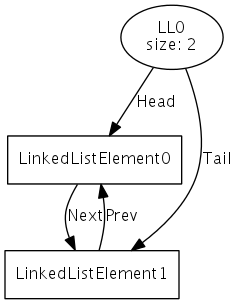
\includegraphics[width=.2\textwidth]{img/ll1}
\label{fig:inst1}
}
\hfil
\subfloat[Instance with $5$ elements for $LinkedList$]{
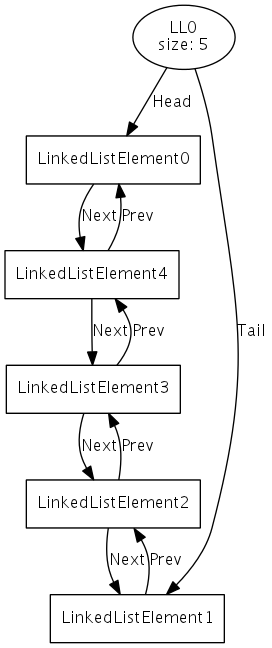
\includegraphics[width=.2\textwidth]{img/ll2}
\label{fig:inst2}}}
\caption{Examples of generated instances from Korat for $LinkedList$ class.}
\label{fig:insts}
\end{figure}

\section{Conclusion}
The conclusion goes here. this is more of the conclusion

\section*{Acknowledgment}
The authors would like to thank...

%\newcommand{\BIBdecl}{\footnotesize{\setlength{\itemsep}{-\baselineskip}}}
\bibliographystyle{IEEEtran}
\bibliography{IEEEabrv,icst12}

\end{document}

